\section{\texorpdfstring{Backgrounds for $\tauTau$}{Backgrounds for tauTau}}
\label{sect:bkg}


\subsection{QCD multi-jet background estimation in tauTau channel}

%In this section, data driven methods are applied to estimate the contribution of
 %  the main backgrounds in the signal region.


In QCD multi-jet events all tau candidates are misidentified as jets. Due to large cross
section and
the poor MC modeling of the tau misidentification rate from jets, the QCD multi-jet contribution in the signal regions is estimated from data using the ABCD" method.

This method indeed relies on different distributions of QCD
in the four exclusive regions labelled as A, B, C (the control regions) and D (the signal region) are defined in a two-dimensional plane as a function of uncorrelated discriminating variables.
In this case the number of QCD events in signal region D can be calculated from the number of QCD events in the control region A multiplied in the ratio of the number of QCD events in the control region C to QCD events in control region B$(T=C/B)$.Figure~\ref{fig:1QCDbg} 

\begin{figure}[htbp]
\centering
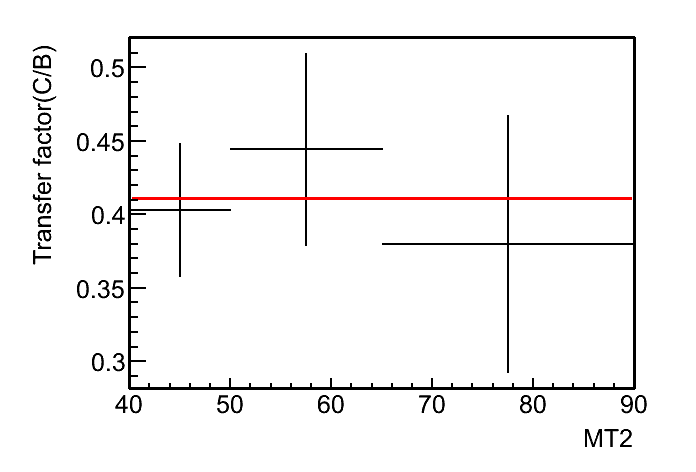
\includegraphics[width=0.49\textwidth]{QCDbginTauTau/Bin1_transferfactor.png}
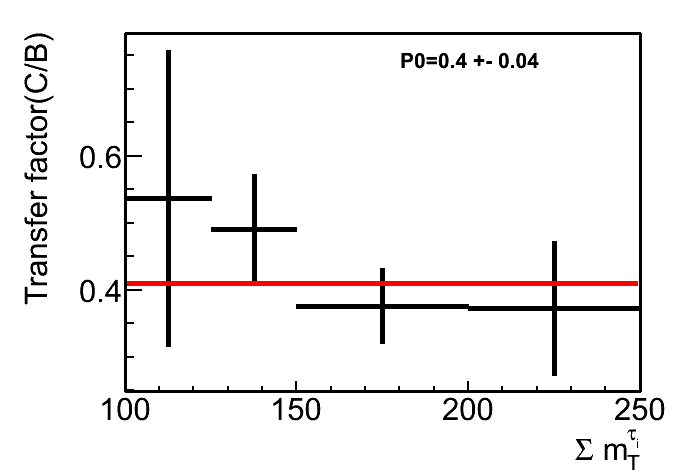
\includegraphics[width=0.49\textwidth]{QCDbginTauTau/Bin2_transferfactor.png} \\
\caption{The ratio of the number of QCD events in the control region C to QCD events in control region B.The
fit line  is drawn in red.
 Left:  $\mttwo>90$ Bin1   Right:  $\SumMT >250$ Bin2.}
\label{fig:1QCDbg}
\end{figure}

The tau identification criterion (tau-id) and a kinematic variable chosen depending (\mttwo in Bini and \SumMT in Binii) 
on the SR are used as the two uncorrelated discriminating variables to define the regions A, B, C and D. The definitions of the control regions are summarized in table \ref{2QCDbg}.

\begin{table}
\begin{center}
\begin{tabular}{|c|c|c|c|}
\hline
Region&A& B & C
\\ \hline\hline
$\mttwo>90$ Bini &$\mttwo >90$ & $\mttwo <90$&$\mttwo <90$ \\
 &at least 1 loose taus&at least 1 loose taus& loose tau veto\\
 &loose-loose loose-medium &loose-loose loose-medium &medium-medium \\
 &loose-tight&loose-tight&medium-tight tight-tight\\ 
 &No cut on charge&No cut on charge& Sum charge==0\\
\hline
$\SumMT>250$ Binii &$\SumMT >250$ &$\SumMT <250$&$\SumMT < 250$\\
 &at least 1 loose taus&at least 1 loose taus& loose tau veto\\
 &loose-loose loose-medium &loose-loose loose-medium &medium-medium \\
 &loose-tight&loose-tight&medium-tight tight-tight\\
 &No cut on charge&No cut on charge& Sum charge==0\\
% &misc.MinMetJetDphiPt40$>$1 is relaxed\\

\hline
\end{tabular}
\caption{The requirement on the kinematic variables used to define the control regions A,B,C.
$\mindphifour>1$ cut is relaxed. }
\label{2QCDbg}
\end{center}
\end{table}

The number of QCD multi-jet events in the control regions is estimated from data after subtraction of other SM contributions estimated from MC simulation.

In order to increase the data statistics, the cut on the $\mindphifour>1$ is relaxed.This cut was
introduced to suppress the QCD background events,now that we want to estimate QCD multi-jet background this cut is relaxed  .The only the ratio this efficiency should be
applied into account QCD in the control regions to estimate the number of QCD events in the signal region.

The fraction of QCD events with all selection cuts with respect to the QCD events with all selection cuts but the
$\mindphifour>1$ are shown in Figure~\ref{fig:3QCDbg} .

\begin{figure}[htbp]
\centering
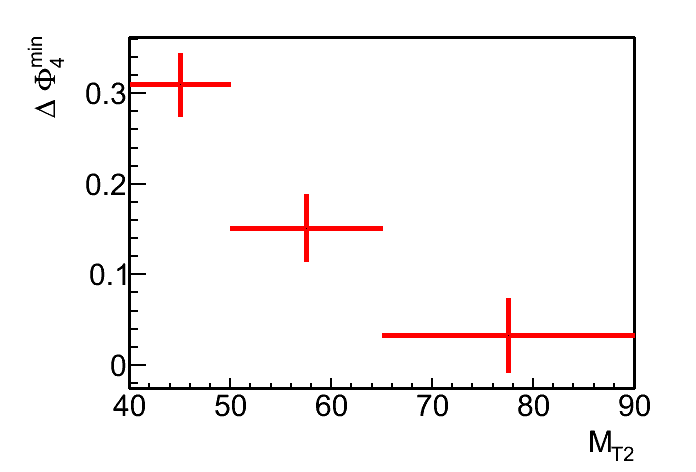
\includegraphics[width=0.49\textwidth]{QCDbginTauTau/Bin1_miscefficiency.png}
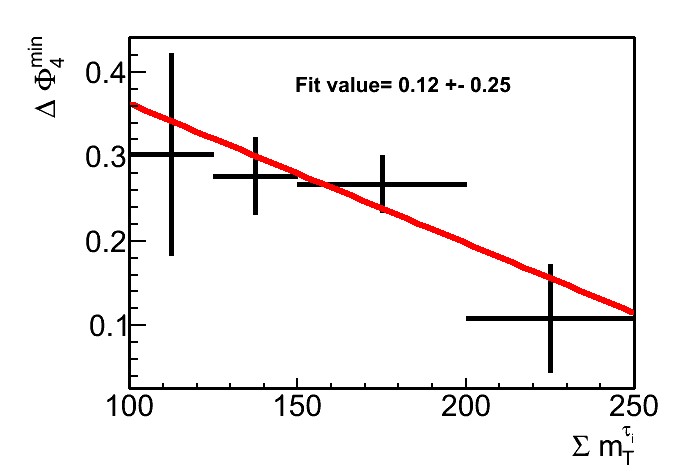
\includegraphics[width=0.49\textwidth]{QCDbginTauTau/Bin2_miscefficiency.png} \\
\caption{ Ratio between QCD multi-jet events passing all selection cuts versus QCD events
 passing all selection cuts but $\mindphifour>1$. Left:  $\mttwo>90$ Bin1   Right:  $\SumMT >250$ Bin2.}
\label{fig:3QCDbg}
\end{figure}




The results of the ABCD method are summarized in table \ref{4QCDbg} and the distributions of the kinematic variables  for data, SM backgrounds and SUSY are shown in the Figure~\ref{fig:5QCDbg}. The SM background distributions
are taken from MC simulation, except for the QCD-multi-jet contribution, which is estimated
using the ABCD method.

\begin{table}
\begin{center}
\begin{tabular}{|l|c|c|c|c|c|c|c|}
\hline
 & Sample & RegionA & RegionB & RegionC & T=C/B & Estimation \\\hline\hline
\multirow{7}{*}{Bini \mttwo$>$90}& Data&10.00 +- 3.16 & 880.00 +- 29.66&  430.00 +- 20.74& \multirow{7}{*}{0.43+-0.32} & \multirow{7}{*}{0.06 +- 0.08}\\ \cline{2-5}

&Z+jets& 2.27 +- 0.90 &29.27 +- 3.22 & 51.45 +- 4.43 & & \\\cline{2-5}

&W+jets& 2.90 +- 1.43&69.20 +- 8.70 &49.25 +- 7.22 & & \\\cline{2-5}

&WW+jets&0.12 +- 0.07 &0.76 +- 0.17 &1.60 +- 0.25 & & \\\cline{2-5}

&Top& 0.49 +- 0.47&21.78 +- 3.13 & 14.51 +- 2.63& & \\\cline{2-5}
&QCD& 4.23 +- 3.62 & 758.99+-31.24& 313.19+-22.55& & \\\cline{2-5}
&Susy& 1.46 +- 0.17& 3.96 +- 0.28& 9.01 +- 0.41& & \\\cline{2-5}
\hline\hline
\multirow{7}{*}{Binii $\SumMT>250$}&Data  &25.00 +- 5.00  &723.00 +- 26.89 &348.00 +- 18.65 & \multirow{7}{*}{ 0.41 +- 0.03} & \multirow{7}{*}{0.61 +- 1.55} &  \\\cline{2-5}

&Z+jets& 2.22 +- 1.07 & 21.78 +- 2.72 & 39.57 +- 3.94& & \\\cline{2-5}

&W+jets&  4.28 +- 1.46&51.84 +- 7.48 & 40.09 +- 6.82& & \\\cline{2-5}

&WW+jets&  0.09 +- 0.05& 0.42 +- 0.13& 0.87 +- 0.19 & & \\\cline{2-5}

&Top&0.42 +- 0.41 &3.07 +- 1.22 & 3.31 +- 1.43& & \\\cline{2-5}
&QCD&18.00 +- 5.33 &645.89+-28.07 & 264.16+-20.30& & \\\cline{2-5}
&Susy& 2.13 +- 0.20&1.18 +- 0.15 &  2.80 +- 0.22& & \\\cline{2-5}
\hline

\end{tabular}
\caption{ The MC predicted backgrounds in the multi-jet control regions, including both the
statistical and systematic uncertainties, and the expected multi-jet contribution,obtained
by subtracting the MC contributions from observed data . Predicted event yields for the
SUSY  in the control regions are also shown. The estimated multi-jet contribution
in the SRs is given in the last column.
}
\label{4QCDbg}
\end{center}
\end{table}


\begin{figure}[htbp]
\centering
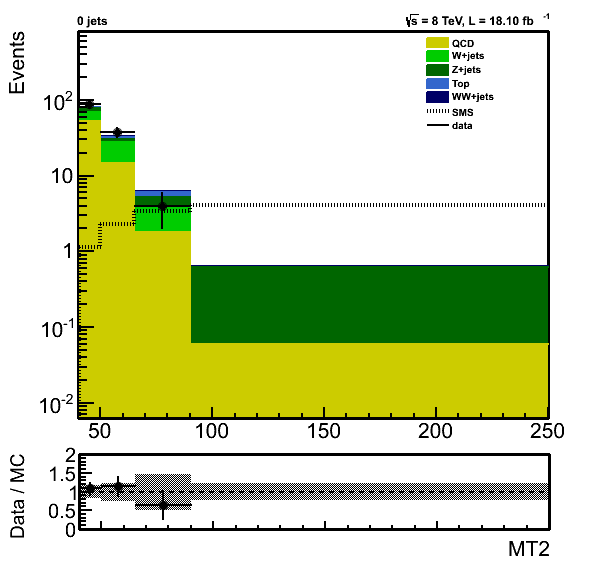
\includegraphics[width=0.49\textwidth]{QCDbginTauTau/Bin1_QCDdatadriven2.png}
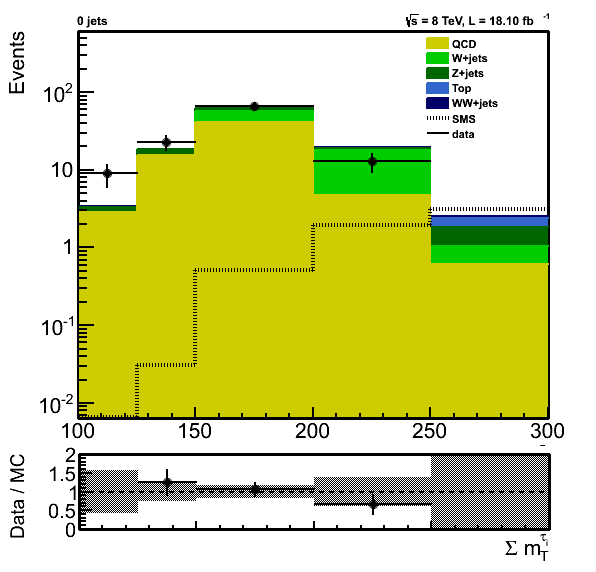
\includegraphics[width=0.49\textwidth]{QCDbginTauTau/Bin2_QCDdatadriven2.png} \\
\caption{Distributions of relevant kinematic variables before the requirement on the given variable
is applied: (a) \mttwo  (b) $\SumMT$ . The QCD multi-jet contribution is estimated from data using the ABCD method.}
\label{fig:5QCDbg}
\end{figure}















